\documentclass[10pt,a4paper]{article}
\usepackage[utf8]{inputenc}
%\usepackage[engl]{babel}
\usepackage[T1]{fontenc}
\usepackage{amsmath}
\usepackage{amsfonts}
\usepackage{amssymb}
\usepackage{graphicx}
\usepackage{bm}
\usepackage[rmargin=1.5cm, lmargin=1.5cm, bmargin=2cm, tmargin=2cm]{geometry}
\usepackage{enumitem}
\setitemize{noitemsep,topsep=0pt,parsep=0pt,partopsep=0pt}


\author{Lars Schiller}
\title{Algorithm for predicting the pose of a gecko-inspired soft robot for a given reference input}


\usepackage{multicol}



\begin{document}


\maketitle

Due to the fact that the behaviour of soft materials is difficult to predict with conventional methods, an algorithm based on a geometric optimization problem is presented.
The algorithm can be used to predict the actual pose of the robot for a given reference input.
Figure~\ref{fig:example} is taken as an example. The initial position is shown in black. 
The individual limbs of the robot have a certain bending angle and all feet are fixed.
Now the torso of the robot should be actuated. 
If only the bending angle of the torso is changed, the grey dashed pose is obtained. 
Obviously, the two rear feet are no longer in the same position. 
Since these feet are fixed, the robot will behave differently in reality. 
In fact, it's much more likely to take up the grey pose. 
Although the bending angles of all limbs have changed, the condition that all feet remain motionless has been fulfilled.

\begin{figure}[h]
\centering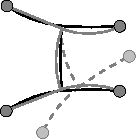
\includegraphics[scale=1]{../Pics/intro/intro.pdf}
\caption{Example Usage}
\label{fig:example}
\end{figure}

In order to let the robot take a pose
%, i.\,e., a position and orientation, 
the user has nine degrees of freedom at his disposal: 
the correspondending pressures $p_i$ for the five bending angles $\alpha_i$ of the limbs $i=1,\dots,5$ and the state of the fixation actuators $f_j \in \{0,1\}$ of the feet $j=1,\dots,4$.
Accordingly, a reference input can be described by
\begin{equation}
\bm{ref} = \left[~ p_1~p_2~p_3~p_4~p_5~f_1~f_2~f_3~f_4~ \right]^\top.
\end{equation}

For the unloaded state, a calibration function can be formulated for each limb, which maps the pressure on the bending angle.
Under load, this function no longer needs to be valid.

\begin{equation}
\alpha_{\textnormal{clb},i} = \textnormal{map}_i(p_i)
\end{equation}

However, this information is not sufficient to describe the robot's actual pose.
%The exact position and orientation of at least one foot must be known.
Experiments have shown that the bending angle of a limb can vary significantly  at the same pressure level due to the softness of the used material. 
The length of a limb can also differ.
In order to describe the pose of the robot, the bending angles $\bm{\alpha}$: 
\begin{equation}
\bm{\alpha} = \left[ \alpha_1~\alpha_2~\alpha_3~\alpha_4~\alpha_5 \right]^\top,
\end{equation}
the actual lengths of the individual limbs $\bm{\ell$}: 
\begin{equation}
\bm{\ell} = \left[ \ell_1~\ell_2~\ell_3~\ell_4~\ell_5 \right]^\top,
\end{equation}
and the orientation of the robot's center point $\varepsilon$ must be known (see Fig.~\ref{fig:model}).
These quantities are defined as the variable to be optimized:
\begin{equation}
\bm{x} = \left[~\bm{\alpha}^\top~\bm{\ell}^\top~\varepsilon~\right]^\top.
\end{equation}

Furthermore, the position of (at least) one fixed foot ($\bm{r}_{j} \in \mathbb{R}^{2 \times 1}$) must be known.
Then, the pose of the robot $\bm{\rho}$, i.\,e. the positions of all feet, can be determined under the assumption of a constant curvature by using the equations \eqref{eq:F1_start}--\eqref{eq:F1_end} if the front left foot is fixed, or the equations \eqref{eq:F2_start}--\eqref{eq:F2_end} if the front right foot is fixed.
The pose can therefore be described as a function of $\bm{x}$ and the position of a fixed foot:

\begin{equation}
\bm{\rho} = \textnormal{fun}\left(\bm{x},~\bm{r}_{j} \right).
\end{equation}


\begin{figure}
\centering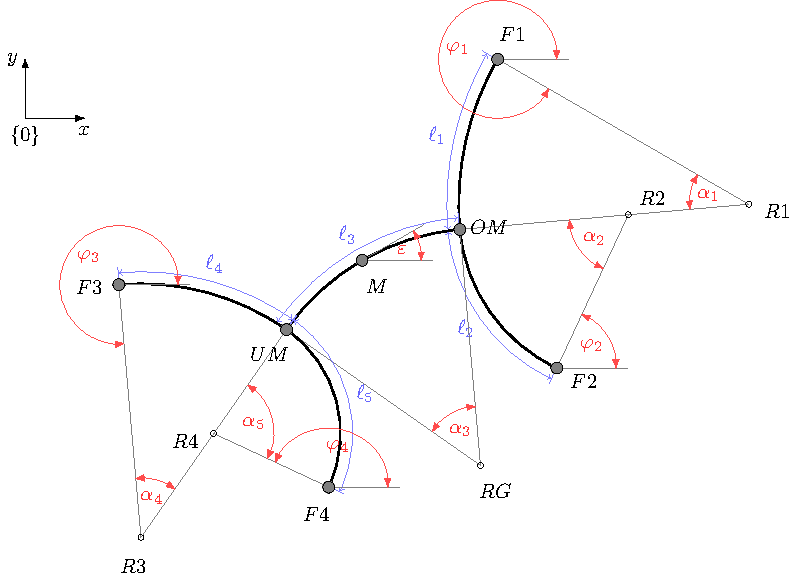
\includegraphics[scale=1]{../Pics/model/model.pdf}
\caption{Nomencalture}
\label{fig:model}
\end{figure}

Here, the pose seems to be independent of the fixed feet.
But the dependency lies in the bending angles and the actual lengths of the limbs. 
These must be determined in such a way that the positions of the fixed feet do not change.
To describe this mathematically, a new index $t$ is introduced, which assigns the quantities to a specific time step.
The new positions of the fixed feet $\bm{r}_{j,t+1}$ are assumed to be the positions from the previous pose $\bm{r}_{j,t}$.
This can be used to define the constraint for the new pose.
All newly fixed feet must have the same position as in the previous step:
%
%So, the new pose is strongly dependent on where the newly fixed feet were in the prior pose.

\newcommand{\mbeq}{\overset{!}{=}}
\begin{equation}
\textnormal{if}~f_{j,t+1}:~~\big|\bm{r}_{j,t+1} - \bm{r}_{j,t}\big|_2 \mbeq 0,
\label{eq:constraint}
\end{equation}

Please note that if this condition is met, at least one foot per time step always remains motionless.
Thus, at least one foot position of the new pose is determined from the beginning and thus dependent on the previous pose.
As a result, all poses of a gait are dependent on the initial position.
%\begin{equation}
%\bm{\rho}_t = \textnormal{fun}\left(\bm{x}_t,~\bm{r}_{j,0} \right).
%\end{equation}



It has already been mentioned that the bending angles $\bm{\alpha}$ and the lengths of the limbs $\bm{\ell}$ are quite variable. 
The orientation angles of the fixation actuators $\varphi_j$ also have a certain margin.
By defining $\bm{\ell}_n = \left[ \ell_{1,n}~\ell_{2,n}~\ell_{3,n}~\ell_{4,n}~\ell_{5,n} \right]^\top$ as the vector containing the nominal length of each limb,
this can be formulated as a objective function:
%\begin{equation}
%obj(\bm{x}) = w_{len}\sqrt{\sum_i \left( \ell_{n,i} - \ell_i \right)^2} 
%+ w_{ang} \sqrt{\sum_i \left( \varphi_i - \alpha_i \right)^2}
%+ w_{ori} \sqrt{\sum_i \textnormal{if}~f_i:~\left( c_{i,j-1} - c_{i, j} \right)^2}
%\label{eq:objective_function}
%\end{equation}

\begin{equation}
obj(\bm{x}_t) = 
  w_{\textnormal{len}}\big| \bm{\ell}_t - \bm{\ell}_n \big|_2
+ w_{\textnormal{ang}}\big| \bm{\alpha}_t - \bm{\alpha}_{\textnormal{clb},t} \big|_2
+ w_{\textnormal{ori}}\sqrt{\sum_j \textnormal{if}~f_{j,t+1}:~\left( \varphi_{j,t+1} - \varphi_{j, t} \right)^2}
\label{eq:objective_function}
\end{equation}
where the weighting factor $w_{\textnormal{len}}$ describes the elasticity of the limbs and $w_{\textnormal{ang}}$ the bending stiffness of the limbs.
The term weighted by $w_{\textnormal{ori}}$ describes the difference between the orientation of the newly fixed feet compared to the orientation in the previous time step.
This can be seen as a dimension for the torsional stiffness of the fixation actuators.
The new pose can now be determined by solving the non-linear optimization problem:

\begin{equation}
\min_{\bm{x}_t \in \mathcal{X}} ~ obj(\bm{x}_t)~~ s.\,t.~ \textnormal{if}~f_{j,t}:~~\big|\bm{r}_{j,t+1} - \bm{r}_{j,t}\big|_2 = 0
\end{equation}
Here  $\mathcal{X}$ describes the set of allowed values.
Each quantity inside $\bm{x}$ has bounds, which are given in the following table:

\begin{center}
\begin{tabular}{c|c|c|c}
var & $\bm{\alpha}$ & $\bm{\ell}$ & $\varepsilon$ \\ 
\hline
bounds & $\left[ \bm{\alpha_{\textnormal{clb}}}-b_{\textnormal{ang}},~\bm{\alpha_{\textnormal{clb}}}+b_{\textnormal{ang}} \right]$ &
$\left[ (1-b_\textnormal{len})\bm{\ell}_n,~(1+b_\textnormal{len})\bm{\ell}_n \right]$ &
$\left[ 0^\circ,~ 360^\circ \right]$
\end{tabular}
\end{center}
These bounds can be tuned with the scalars $b_{\textnormal{ang}}$ and $b_{\textnormal{len}}$.
For solving the problem, for example the \texttt{SLSQP}-Algorithm provided by the python package \texttt{scipy} can be used.


\clearpage
\begin{multicols}{2}

Coordinates for $F1$ fixed:

\begin{equation}
r_i = \frac{360 ~ \ell_i}{2 \pi ~ \alpha_i},~~ \textnormal{for}~ i \in [1,2,3,4,5]
\end{equation}

\begin{equation}
c_2 = c_1 + \alpha_1 + \beta_1
\label{eq:F1_start}
\end{equation}

\begin{equation}
c_3 = 180 + \gamma + \alpha_2 + c_1 + \alpha_1
\end{equation}

\begin{equation}
c_4 = 180 + \gamma + \alpha_1 - \beta_2 + c_1
\end{equation}


\begin{equation}
R1 =  \begin{bmatrix} 
F1_x +\cos(c_1)~r_1 \\ 
F1_y + \sin(c_1)~r_1\end{bmatrix}
\end{equation}

\begin{equation}
OM =  \begin{bmatrix} 
R1_x - \sin(90-c_1-\alpha_1)~r_1 \\ 
R1_y - \cos(90-c_1-\alpha_1)~r_1 \end{bmatrix}
\end{equation}

\begin{equation}
RG =  \begin{bmatrix} 
OM_x + \cos(90-c_1-\alpha_1)~r_\gamma \\ 
OM_y - \sin(90-c_1-\alpha_1)~r_\gamma \end{bmatrix}
\end{equation}

\begin{equation}
UM =  \begin{bmatrix} 
RG_x - \cos(\gamma - 90 + c_1 + \alpha_1)~r_\gamma \\ 
RG_y - \sin(\gamma - 90 + c_1 + \alpha_1)~r_\gamma \end{bmatrix}
\end{equation}

\begin{equation}
R4 =  \begin{bmatrix} 
UM_x + \sin(\gamma - 90 + c_1 + \alpha_1)~r_4 \\
UM_y - \cos(\gamma - 90 + c_1 + \alpha_1)~r_4 \end{bmatrix}
\end{equation}

\begin{equation}
F4 =  \begin{bmatrix} 
R4_x + \sin(-c_4-90)~r_4 \\
R4_y + \cos(-c_4-90)~r_4 \end{bmatrix}
\end{equation}

\begin{equation}
R3 =  \begin{bmatrix} 
UM_x + \sin(\gamma - 90 + c_1 + \alpha_1)~r_3 \\
UM_y - \cos(\gamma - 90 + c_1 + \alpha_1)~r_3 \end{bmatrix}
\end{equation}

\begin{equation}
F3 =  \begin{bmatrix} 
R3_x - \cos(-c_3)~r_3 \\
R3_y + \sin(-c_3)~r_3 \end{bmatrix}
\end{equation}


\begin{equation}
R2 =  \begin{bmatrix} 
OM_x + \cos(c_1 + \alpha_1)~r_2 \\
OM_y + \sin(c_1 + \alpha_1)~r_2 \end{bmatrix}
\end{equation}

\begin{equation}
F2 =  \begin{bmatrix} 
R2_x + \sin(c_2 - 90)~r_2 \\
R2_y - \cos(c_2 - 90)~r_2 \end{bmatrix}
\label{eq:F1_end}
\end{equation}

\columnbreak


Coordinates for $F2$ fixed:

\begin{equation}
c_1 = c_2 - \alpha_1 - \beta_1
\label{eq:F2_start}
\end{equation}

\begin{equation}
c_3 = 180 + \gamma - \beta_1 + \alpha_2 + c_2
\end{equation}

\begin{equation}
c_4 = 180 + \gamma - \beta_2 + c_2 - \beta_1
\end{equation}


\begin{equation}
R2 = \begin{bmatrix}
F2_x - \sin(c_2 - 90)~r_2 \\
F2_y + \cos(c_2 - 90)~r_2
\end{bmatrix}
\end{equation}

\begin{equation}
OM = \begin{bmatrix}
R2_x - \sin(90- c_2 + \beta_1)~r_2 \\
R2_y - \cos(90- c_2 + \beta_1)~r_2
\end{bmatrix}
\end{equation}

\begin{equation}
RG = \begin{bmatrix}
OM_x + \cos(90- c_2 + \beta_1)~r_\gamma \\
OM_y - \sin(90- c_2 + \beta_1)~r_\gamma
\end{bmatrix}
\end{equation}

\begin{equation}
UM = \begin{bmatrix}
RG_x - \cos(\gamma - 90 + c_2 - \beta_1)~r_\gamma \\
RG_y - \sin(\gamma - 90 + c_2 - \beta_1)~r_\gamma
\end{bmatrix}
\end{equation}

\begin{equation}
R4 = \begin{bmatrix}
UM_x + \sin(\gamma - 90 + c_2 - \beta_1)~r_4 \\
UM_y - \cos(\gamma - 90 + c_2 - \beta_1)~r_4
\end{bmatrix}
\end{equation}

\begin{equation}
F4 = \begin{bmatrix}
R4_x + \sin(-c_4 -90)~r_4 \\
R4_y + \cos(-c_4 -90)~r_4
\end{bmatrix}
\end{equation}

\begin{equation}
R3 = \begin{bmatrix}
UM_x + \sin(\gamma - 90 + c_2 - \beta_1)~r_3 \\
UM_y - \cos(\gamma - 90 + c_2 - \beta_1)~r_3
\end{bmatrix}
\end{equation}

\begin{equation}
F3 = \begin{bmatrix}
R3_x - \cos(-c_3)~r_3 \\
R3_y + \sin(-c_3)~r_3
\end{bmatrix}
\end{equation}


\begin{equation}
R1 = \begin{bmatrix}
OM_x + \sin(90-c_2+\beta_1)~r_1 \\
OM_y + \cos(90-c_2+\beta_1)~r_1
\end{bmatrix}
\end{equation}


\begin{equation}
F1 = \begin{bmatrix}
R1_x - \sin(90-c_1)~r_1 \\
R1_y - \cos(90-c_1)~r_1
\end{bmatrix}
\label{eq:F2_end}
\end{equation}

\end{multicols}




\end{document}